\chapter{Unsupervised Learning}\label{ch_unsupervised}
\chapterauthor{Jeff Yoshimi}

\section{Introduction}

Unsupervised learning is learning without a teacher. It is a method for changing the weights of a network without telling a network what we want it to do (that is, without consulting target data or ``labels''; see chapter \extref{ch_data_science}). You set a neural network loose in an environment (which usually means exposing it to a bunch of samples from a table of input vectors) and see what it comes up with. How can a neural network adapt to an environment on its own, without being told what to do?  How can it ``self-organize''? Given how often animals find themselves in this situation---of not having a teacher around---it's an important topic.\footnote{Of course, animals do experience unconditioned rewards and punishments and their learning is in that sense ``supervised.'' Skinner famously thought this was enough to explain all animal behavior, and this is the basis of reinforcement learning (RL) approaches. So that form of supervised learning still has a chance, though RL researchers often also draw on unsupervised methods.} It turns out that unsupervised learning algorithms are quite powerful, both as engineering tools in machine learning and also as a way of modeling the development of certain types of neural circuits and psychological capacities.

We begin the chapter with a discussion of Hebb's rule, a classic associative learning rule that allows us to associate paired stimuli. We consider how Hebb's rule and its variants can be used to create feed-forward pattern associators. We then consider how a Hebbian-type rule (Oja's rule) allows layered networks to achieve dimensionality reduction, where one layer extracts the most statistically important information from the previous layer. Finally, we review competitive learning algorithms that can be used to associate output neurons with clusters in an input space. This culminates in a discussion of self-organizing maps, which can be used to model certain features of the cerebral cortex and can also be used as a machine learning tool.\footnote{There is a lot more to unsupervised learning than what is covered here. For an overview in the context of machine learning, see \url{http://scikit-learn.org/stable/unsupervised_learning.html}.}  In chapter \extref{ch_unsupervised_recurrent}, we consider how unsupervised methods can be used to train recurrent networks.
% More refs to this, including in Oja. https://grey.colorado.edu/CompCogNeuro/index.php/CCNBook/Perception

\section{Hebbian Learning}

% Use prime notation here for next time step, or else remove that notation in next chapter.
% Add something about learning as dynamics on weight space. Reminder that weights are parameters for a dynamical system.

Learning in a neural network corresponds to adjustment of its weights by application of a \glossary{learning rule}. A learning rule is a method for updating the weights of a neural network over time. It is the counterpart to an activation function (chapter \extref{ch_act_functions}), but it acts on the weights between nodes rather than on the activation levels of the nodes.  Some learning rules are visible in Simbrain by editing a weight and consulting the \emph{update  rule} drop-down box.

A learning rule for weight $w_{j,k}$  can be written as a delta value,
$\Delta w_{j,k}$, meaning ``change in strength of weight $w_{j,k}$'' (the symbol $\Delta$ is often used to describe changes in a variable). At any
time step, you simply add the current value of $\Delta w_{j,k}$ to the weight's 
current strength to get the weight's new strength at the next time step. If we let a prime symbol $\prime$ indicate the next time step, then we have this rule:
\begin{eqnarray*}
w^\prime_{j,k} = w_{j,k} + \Delta w_{j,k}
\end{eqnarray*}
It's quite simple. The strength of the weight $w_{j,k}$ at the next time step will be equal to its current value plus some delta value. It's just addition. For example, if $w_{1,4} =-1$ and $\Delta w_{1,4} = 4$, then $w^\prime_{1,4}  = -1 + 4 = 3$. 
% For convenience we will drop the prime symbol, since context will usually make it clear what the updated weight value is.

Hebbian learning is one of the oldest and simplest learning algorithms for neural networks. It is biologically plausible (it is based on Long Term Potentiation, discussed in chapter \extref{ch_neuro}) but has limitations that prevent it from being widely used in its basic form (variants of the Hebb rule are, however, widely used). 

The basic idea of Hebbian learning is that when connected neurons are both active, the weight connecting them is strengthened. You know the slogan: ``neurons which fire  together, wire together.'' Donald Hebb proposed this idea in the 1940s, before there was experimental  support for it. As he put it:
\begin{quote}
When an axon of cell A is near enough to excite a cell B and repeatedly or persistently takes part in firing it, some growth process or metabolic change takes place in one or both cells such that A's efficiency, as one of the cells firing B, is increased \cite{hebb2005organization}.
\end{quote}

Formally,  the Hebb rule states that the change in a weight $w_{j,k}$ at a time is 
equal to the product of a \glossary{learning rate} $\epsilon$, the source node's 
activation $a_k$, and the target node's activation $a_k$. 
\begin{eqnarray*}
\Delta w_{j,k} = \epsilon a_j a_k
\end{eqnarray*}
The learning rate $\epsilon$ controls the rate at which the weights change each time the rule is applied (each time we press ``step'' in Simbrain). If we set $\epsilon=0.00002$, the weights will change very slowly. If we set $\epsilon=10$, they will change very quickly. Note that we can \emph{stop} learning by setting $\epsilon=0$ (in which case $\Delta w_{j,k}$ will always be 0). Most of the learning algorithms we consider will have some sort of learning rate. Learning rates are usually set between $.01$ and $1$.

% If not clamped, then at each time step the activations change too, so the computation is more complex
When nodes $j$ and $k$ are clamped (so that their activations can't change), the rule is especially easy to apply. It is simply the product of the two nodes' activations times the learning rate. If both neurons have an activation of 1, then at each time step we simply add the learning rate to the weight. For example, if $a_j = 1, a_k=1, \Delta w_{j,k} =1$ , then at time step the weight strength will increase by 1.  If $a_j = 1, a_k=1, \Delta w_{j,k}= .5$, then at time step the weight strength will increase by .5.

Notice that if both the source and target node activations of a Hebbian weight are positive, then the weight's value will increase (they ``fire together'' so they ``wire together''). If one activation is positive and one is negative, the weight will decrease. If both activations are negative, they will also increase (since a negative number times a negative number is positive).\footnote{The negative-positive and negative-negative cases are biologically implausible but still useful in many algorithms.}  If either activation is 0, the weight will not change, which is an important baseline case: neurons that \emph{don't fire}, don't wire! Most our neurons are quiet most of the time, and thus the synapses connected to them don't change. 

Making a simple Simbrain network to test and explore these ideas is easy. Create two nodes and connect them with a weight. Double click on the weight, set its update rule to Hebbian, and set the learning rate to whatever you desire. Clamp both nodes. Now when you run the network, you will see the weight change: it gets larger when both nodes are negative or positive, and lower when one node is negative and the other is positive. The rate of change is set by the learning rate. The weight will generally just ``explode'', i.e. increase or decrease indefinitely. In Simbrain, the weight strengths are bounded, so they will often just race towards these bounds. 

% Use "exercise" format. (Do same in next two chapters?  And back in DST chapter too?). 

\bigskip

\noindent
{\bf Example 1.} Suppose we have two nodes with activations $a_1$ and $a_2$, and that the activations of the nodes are clamped. Further suppose we have \\ \\
\indent \qquad\qquad The activations on the nodes: $(a_1,a_2) = (1,2)$\\
\indent \qquad\qquad The weight: $w_{1,2} = -1$ \\ \\
and that the learning rate is $\epsilon =0.5$. What will the value of the  weight be after three time steps? 

First, we compute $\Delta w_{1,2}$, the  amount that the weight will change at each time step:
\begin{eqnarray*}
\Delta w_{1,2} = \epsilon \cdot a_1 \cdot a_2 = (0.5)(1)(2) = 1
\end{eqnarray*}
The value of $\Delta w_{1,2}$ never changes because the activations are 
clamped. So the weight of $w_{1,2}$ will change by $\Delta w_{1,2} = 1$ for
each of the time steps. Since $w_{1,2}$ begins at $-1$, it will be $0$ after 
the first time step, it will be $1$ after the second time step, and it will be 
$2$ after the third time step. {\bf Answer:} $w_{1,2} = 2$.

\bigskip

\noindent
{\bf Example 2} You can see from the previous example that over time the weights will 
go towards extreme values with the Hebb rule. This is a problem with Hebbian 
learning: it tends to push weights towards positive or negative infinity. One way to slow 
this down is to use a smaller value for $\epsilon$. Suppose in example 1 that
$\epsilon =  0.01$. What would the values for the weight be at each time step?
{\bf Answer:} Time 1: $w_{1,2} = -0.98$, Time 2: $w_{1,2} = -0.96$. Time 3:  $w_{1,2} = -0.94$.

\section{Hebbian Pattern Association for Feed-Forward Networks}\label{ff_associator}

% Citations
A classic use of the Hebb rule is to model pattern association. The underlying idea is simple: when an agent perceives multiple stimuli at the same time or nearly the same time (what the classical British empiricists discussed in chapter \extref{ch_history} called ``contiguity in time and place''), we tend to associate them. If you often hear a song while being around some person, you may come to associate the two. The song may later remind you of that person.\footnote{Associations like these are a common literary theme. Marcel Proust's epic \emph{Remembrance of Things Past} is a thousands-of-pages long novel that begins with memories inspired by the smell of a cookie, a ``crumb of madeleine'' \cite{proust2006remembrance}. Gabriel Garc\'{i}a M\'{a}rquez's \emph{Love in the Time of Cholera}, opens with ``It was inevitable: the scent of bitter almonds always reminded him of the fate of unrequited love.''}  If a dog hears a bell just before receiving food, it will associate the two. Thus classical conditioning can, to a first approximation, be explained by the Hebb rule.\footnote{\label{hebb_updated}An actual model of the conditioning is the Rescorla Wagner model, which influenced the development of similar models in reinforcement learning. Both can be explored in Simbrain. See the scripts \emph{rescorlaWagner.bsh} and \emph{actor\_critic.bsh}.}   But we will see that simple Hebbian pattern associators are problematic, so the rule must be supplemented in various ways.\footnote{\label{grayArea} It should be noted that Hebbian pattern associators (especially feed-forward pattern associators) are really in a gray area between unsupervised and supervised learning. They are unsupervised in that there is no explicit teacher. However, in practice, we often clamp the nodes of these network using desired outputs. From an unsupervised perspective, we can think of this as values that were set ``by nature'' (e.g. the sound of a song in one neural population, and sight of a friend in another neural population), so it can still be thought as unsupervised, and it is still the case that there there is no explicit training signal. Also, the Hebb rule is a natural place to start in our study of unsupervised learning. So we cover Hebbian pattern associators here, even though they are on the cusp between the two types of learning.}
% A reference to PDP 1 example and Simbrain simulations. 

% In just about every case, the Hebb rule is just applied once or a few times and then the weights are frozen. This is the case in Hopfield for example.

% Some more prominent picture or something is needed here to call attention to the functions

We begin by considering pattern association in feed-forward networks. Feed-forward networks can be thought of as functions that take a vector (a list of numbers; see chapter \extref{ch_linear_algebra}) as input and produce a vector as output. A multiple layered feed-forward network computes a series of vector-to-vector transformations based on the intervening weights (which, recall, can be represented by weight matrices).\footnote{Recall from algebra that a function is a rule that associates objects (usually numbers) in a domain with unique objects (usually other numbers) in a range. For example $f(x) = x^2$ associates real numbers with positive real  numbers: $f(2) = 4$, $f(-1) = 1$, and $f(0) = 0$. We can also think of feed-forward neural networks as  computing functions, which associate input vectors with output vectors. For example, a network with 3 input nodes and 3 output nodes takes 3-dimensional input vectors with 3 dimensional output vectors. It can be thought of as a rule which associates vectors in a three-dimensional vector space with vectors in another three-dimensional vector space.} As the weights in this network change, the way it associates input vectors with output vectors changes. That is, the function associated with a feed-forward neural network changes as its weights change. 

The Hebb rule can be used to train a feed-forward network to learn a set of pattern associations, and thereby to approximate a function between a set of input vectors and a set of output vectors. The basic idea is simple. We simply set the (clamped) input and output nodes to the patterns we desire, and then apply the rule. 

Suppose we want to use the Hebb rule to train a network to learn the following three associations:
\begin{itemize}
\item $(1,0,0) \rightarrow (1,.4)$
\item $(0,1,0) \rightarrow (.8,.3)$
\item $(0,0,1) \rightarrow (.5,.7)$
\end{itemize}

Something like this can occur in the brain. We can imagine that one population of neurons receives one kind of input (e.g. auditory signals from a song, or olfactory signals from a bowl of bitter almonds) and another part of the brain receives another kind of input (e.g. visual inputs corresponding to a person). The Hebb rule says that since these two populations of neurons are both firing at the same time, an association should form between the two patterns. I often smell bitter almonds when around that person, so later, when I am around bitter almonds again, it arouses a visual memory.

To build this kind of model in Simbrain, take the following steps:

(1) Create the network. Follow the template shown in figure \ref{ffAssociator}. Make all the neurons clamped, the output neurons linear, and set all weights to Hebbian with a learning rate of 1. Also, initialize the weights to a value of 0 by pressing $w$ then $c$. 

(2) Train the network. Set the input and output nodes to their desired values. Now iterate Simbrain once. The weights will be updated according to the Hebb rule, and our first association has been formed. You will notice the synapses change color and size. Repeat this process exactly once for each association.

\begin{figure}[h]
\centering
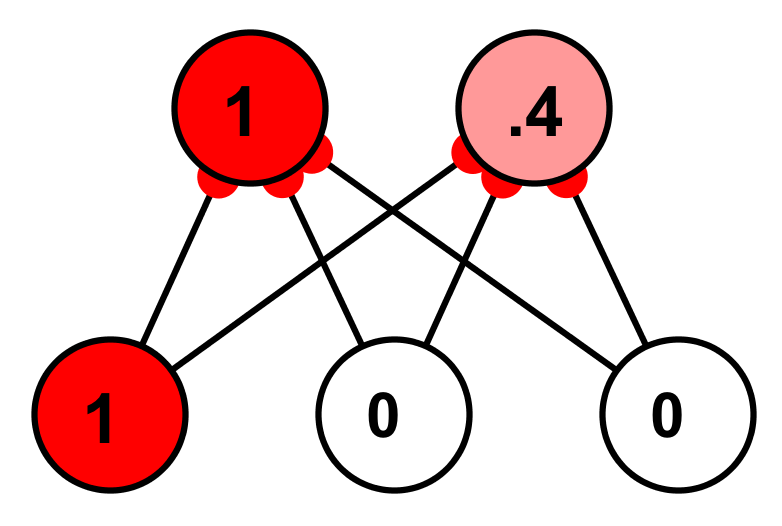
\includegraphics[scale=.4]{./images/net-3-2.png}
\caption[Simbrain screenshot.]{Learning one association in a feed-forward network using the Hebb rule.}
\label{ffAssociator}
\end{figure}
% Label the nodes in some meaningful way.

(3) Test the network's ability to recall patterns.  Now we want to test the network to see how well it can recall these associations. Will it recall the right target pattern given a source pattern? Has it properly implemented the vector-valued function above?  To test the network, we need to do two things. First, we must unclamp the output neurons. Second, we must stop the weights from changing by clamping them (a \glossary{clamped weight} is the same as a clamped node; when weights are clamped, their value no longer changes). Now we are ready to test. For the first input pattern, set the input nodes to $(1,0,0)$, and iterate the workspace. The output neurons should produce the correct pattern, $(1, .4)$. Similarly for the other input-output pairs.

Notice that the Hebbian pattern associator associates localist category vectors (one-hot vectors) with distributed feature vectors. This is similar to what is sometimes called a \glossary{generative model}, that is, a model that can be used to generate prototypical features given a category label.  But for the rest of this chapter we will ``reverse'' the situation, focusing on \glossary{discriminative model}s that associate distributed feature vectors with one-hot categorical or localist vectors. (On generative vs. discriminative models see chapter \extref{ch_data_science}).

The simple Hebb rule, used as a pattern associator, is extremely brittle. Consider the following drawbacks of the method we used to train the associator.

First, we had to carefully clamp and unclamp the nodes and weights in a sequence. In fact, the method we used is almost like a form of supervised learning (chapter \extref{ch_supervised}), because we carefully set the output nodes to target values. In a living network, no such clamping and unclamping occurs. The learning just happens automatically. 

Second, we only updated once. If we had kept running the network, the weights would keep getting larger and the correct associations would have been wiped out. 

Third, we used \glossary{orthogonal} input vectors. Recall from chapter \extref{ch_linear_algebra} that orthogonal vectors have a dot product of 0. For example, $(1,0)$ and $(0,1)$ are orthogonal because $(1,0) \cdot (0,1) = 1 \times 0 + 0 \times 1 = 0$. One-hot encodings (see chapter \extref{ch_data_science}), where just one node is on and the others are off, are an easy way to obtain orthogonal inputs. One-hot input vectors give rise to learning on \emph{completely different weights}. The vector $(1,0,0)$ only changes the weights fanning out from the first input node. The  vector $(0,1,0)$ only changes weights fanning out from the second node. On the other hand, if input vectors are {\em not} orthogonal, then they interfere with one another and we are no longer guaranteed perfect recall. This is sometimes called \glossary{cross talk}. To see this, try repeating the example just given, but using input vectors $(1,1,0)$, $(0,1,1)$ and $(1,1,1)$. You will not get good results, because the input vectors overlap. In general, the degree of cross-talk in Hebbian pattern association  is proportional to how similar the input vectors are.\footnote{For a more detailed discussion, see \cite{fausett1994fundamentals}, p. 105.}
% Add a more detailed statement of conditions of perfect recall, which are in Fausett.
% Mention catastrophic interference, since Dave talks about it in his course?

In practice, more robust variations on Hebb's rule are required to model conditioning and associative learning (see note \ref{hebb_updated}). But this example still gives a flavor of how Hebbian learning works and what it can do.

\section{Oja's Rule and Dimensionality Reduction Networks}

% See Talking Nets, p. 256.

We have seen that the Hebb rule tends to make weights explode to their maximum or minimum values. One solution to this problem is to update all the fan-in weights on a node together, and to update them using Hebb's rule and then rescale the weights so that they sum to 1 (see chapter \extref{ch_data_science}); this is sometimes called ``renormalizing'' the weights). This prevents the weights from ``blowing up'' and means that what matters in a set of weights is just the \emph{relative} size of each weight. This kind of computation can also be done locally. This is done using Oja's rule.\footnote{The formula is $\Delta w_{j,k} = \epsilon a_k (a_j - a_k  w_{j,k})$.}

One thing that Oja's rule can do is dimensionality reduction. Recall from chapter \extref{ch_linear_algebra} that dimensionality reduction is a way of taking high dimensional data and representing it, usually with some distortion, in a lower dimensional space. We have seen how dimensionality reduction helps us to analyze data from neural networks. But it turns out that feed-forward neural networks can also \emph{implement} dimensionality reduction. Suppose you have a feed-forward network with 3 input nodes and 1 output node. This is a form of dimensionality reduction!  It's a way of taking vectors in a space (the input space) and projecting them to a lower dimensional space (the output space). We can call feed-forward networks where there are more input nodes than output nodes \textbf{dimensionality reduction networks}. A random 3-1 network might  not do any significant type of dimensionality reduction, but it does take a set of points in a 3-dimensional input space, and for each of them produce some point in a 1-dimensional output space. So we have a 3-1 dimensionality reduction network. 
% Citation to use of neural networks to do dimensionality reduction

\begin{figure}[h]
\centering
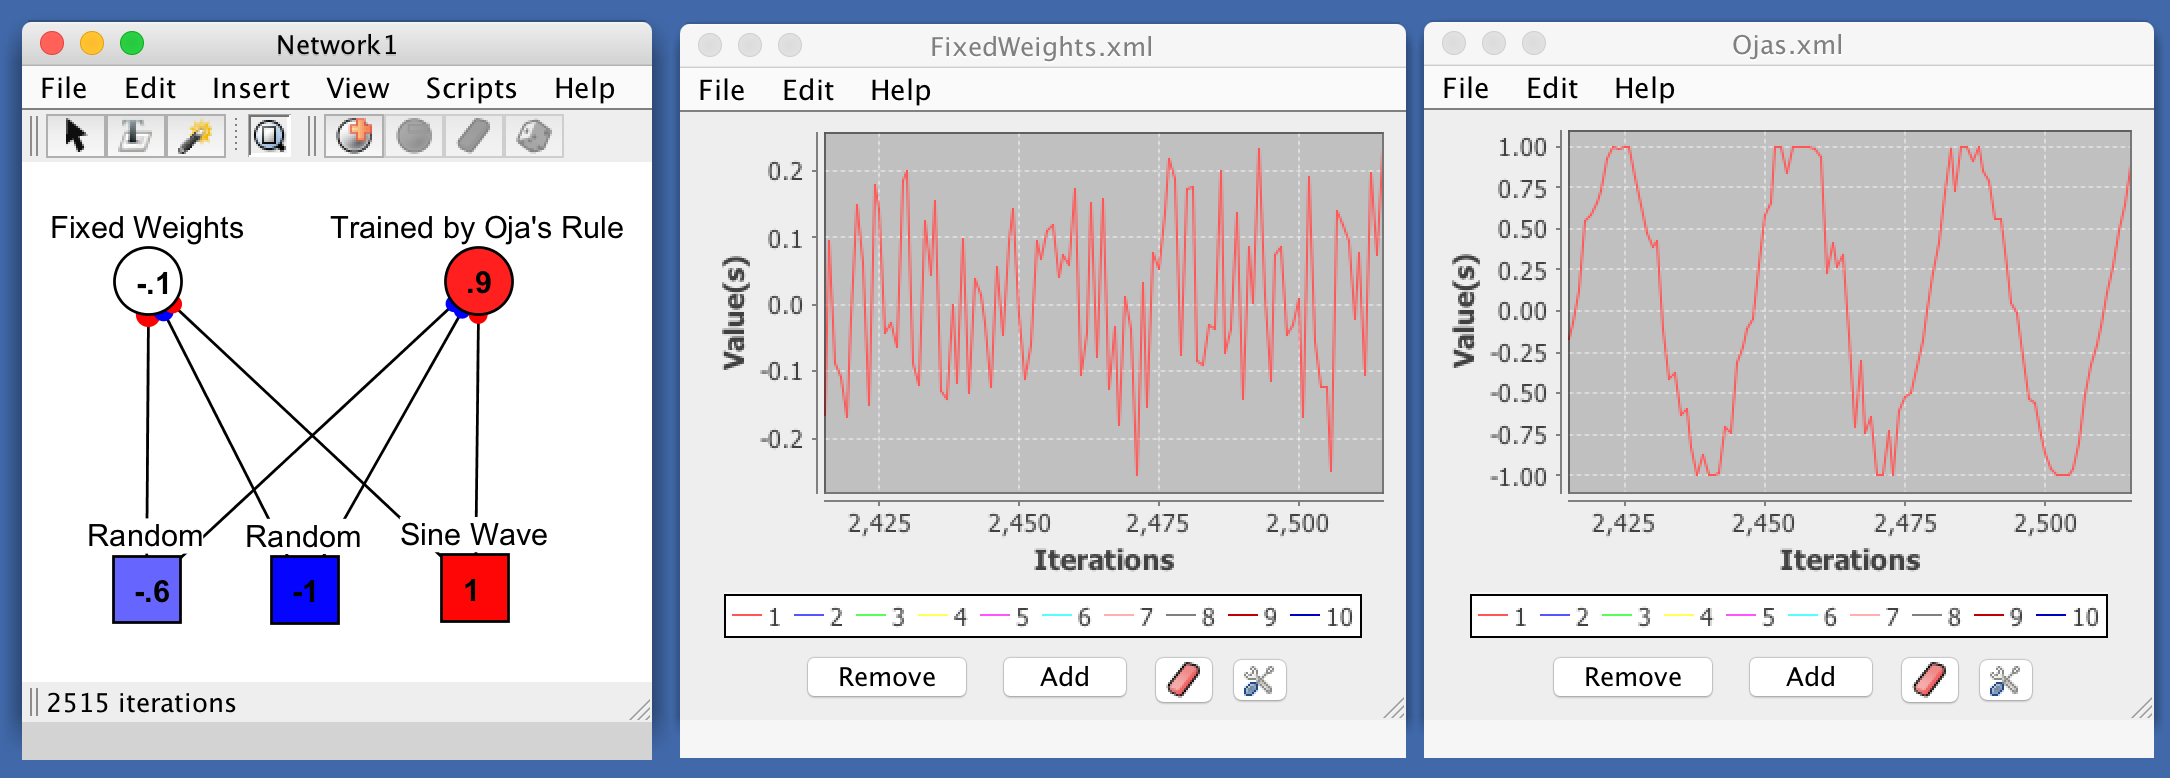
\includegraphics[scale=.4]{./images/OjasRule.png}
\caption[Simbrain screenshot]{An illustration of Oja's rule for dimensionality reduction. Two of the input nodes produce random noise, and the third produces a sine wave. Think of each output node as performing a 3-to-1 dimensionality reduction. The output node on the left was initialized with fixed random weights that don't change. The output node on the right has weights trained by Oja's rule. Time series for two output nodes are shown in the middle and right panels. Notice that the node with weights trained by Oja's rule extracts the sine wave, which is the most informative part of the 3-dimensional input signal.}
\label{oja_dim_reduction}
\end{figure}

When Oja's rule is used on a set of fan-in weights, the resulting network performs a meaningful type of dimensionality reduction, specifically PCA (Principle Components Analysis).\footnote{Some background on PCA and how it works, and some of the other dimensionality reduction methods included with Simbrain, is here: \url{http://hisee.sourceforge.net/about.html}.}   This is the same method used by default in the Simbrain projection component, so it is something you may already have some intuitive familiarity with. 

An example illustrating one use of Oja's rule is shown in Fig. \ref{oja_dim_reduction}. Two of the input activity generators produce random values, and the third produces a sine wave. In the 3-dimensional input signal the output nodes are receiving, the sine wave is the principal part. We'd like to be able to recover just the sine wave. That's what Oja's rule does to the extent that it implements PCA. The output node on the left has fixed random weights. The output node on the right has weights trained by Oja's rule. Think of these as two 3-to-1 dimensionality reduction networks. Notice that the time series plot of the activation of the node on the right shows the sine wave, but the time series plot on the left does not.

Something like this may be what's happening in the human brain. Hebb-like learning rules  have been shown to operate in the brain (LTP, LTD, STDP, etc.; see chapter \extref{ch_neuro}). Moreover, it is known that successive layers of cortical network extract increasingly refined and informative signals from preceding layers. Something like Oja's rule might be at work during this extraction, but it remains an open question.

% Sanger / generalized Hebb rule
% Relation to information theory

\section{Competitive learning}

% Add ML types of thing, like k-means, in part to sync with the python assignments in the course

We now consider a second general type of unsupervised learning, \glossary{competitive learning}, where networks automatically detect statistical tendencies in an input environment. The Hebb rule was able to pick up associations between inputs and outputs automatically, but it was brittle. Competitive learning is much more robust, and it works in a purely unsupervised way (with the Hebb rule we imagined something else was setting the output values of the network).

Competitive networks are feed-forward networks where each output node ``competes'' with the others to represent a certain class or ``cluster'' of inputs in the input space. For example, in a world of cheese and flowers, a competitive network will automatically learn to represent cheeses and flowers with different nodes, without being told about the difference  (see Fig. \ref{competitive_3}). It just develops a sense over time that cheese and flowers are different. 

Something like this also happens in the brain. Neurons automatically come to represent features of an animal's sensory environment over time, even without a teacher. For example, neurons in the visual cortex learn to respond to specific types of edges, and neurons in auditory cortex learn to respond to specific frequencies of sound. They do this without targets, labels, or ``desired outputs''; they learn to represent these features only based on the input dataset provided by nature.\footnote{Although it is worth noting that plausible feature detectors in the brain can also be developed using supervised learning, as with the deep network shown in figure \extref{deepLearning_Vision}  in chapter \extref{ch_neuro}.}

In machine learning, clustering algorithms do something similar to competitive networks, automatically detecting clusters of similar input vectors in an input space.\footnote{This is how algorithms like k-means and dbscan work; see \url{http://scikit-learn.org/stable/modules/clustering.html}.} I like the example of a streaming movie service like Netflix. Netflix can look at  a lot of movies, code the movies as vectors (which contain attributes about each movie and who tends to watch that movie). Then they can run an unsupervised clustering algorithm to automatically lump similar movies together. Then the people at Netflix can hand-label those clusters, with names like ``Zombie Horror'', ``Quirky romance'', and ``Drama with a strong female lead.''

\subsection{Simple Competitive Networks}

% Add Rummelhart/Zipsher quotes
There are different approaches to competitive learning, both in machine learning and cognitive science. We begin with simple competitive networks, which can be easily created in Simbrain using \emph{insert $>$ network $>$ competitive}, or by opening a workspace or script that begins with ``competitive.''

Recall from chapter \extref{ch_linear_algebra} that the input nodes of a network define an input space, which corresponds to the set of all patterns (input vectors) that could occur on those nodes. Each pattern of activations over the input nodes of a network is a point in its input space. Often these sets of input vectors have some structure: in a smell network, for example, objects that produce similar odors will produce similar input vectors, which correspond to ``clustered'' points in the input space. 

A competitive network will automatically learn to represent these clusters. The key idea that makes this possible is the fact that {\it the input space has the same number of dimensions as the fan-in weight space for each output node}. For example, in Fig. \ref{competitive_3}, the input space is 5-dimensional, and each of the three output nodes has a fan-in weight vector with 5 weights. Thus, each of the fan-in weight vectors can be represented in the same 5 dimensional input space. As the network learns, the fan-in weight vectors are updated in such a way that they become closer to specific clusters of inputs. In this way, different output nodes come to respond to different clusters of inputs. Thus, the output nodes are trained to be \emph{cluster detectors}.
% Fan-in also called  a ``reference'' or ``codebook vector'' for the output node or the class the output node represents (Fausett, p. 187) \cite{fausett1994fundamentals}. ``The weight vector for an output unit in a clustering net...serves as a representative, or exemplar, or code-book vector for the input patterns which the net has placed on that cluster'' (p. 157).

The basic idea is shown in Fig. \ref{competitive_3} and Fig. \ref{competitiveInputSpace}. Each time the agent smells an object, a pattern of activity occurs over its 5 nodes, which is a point in a 5-dimensional input space. We can project these points to 2 dimensions, and then view them as in Figure \ref{competitiveInputSpace}. Each point corresponds to one smell.\footnote{We could also use a table of inputs, in which case each row of the table, each sample, would be a point. This is how competitive learning is usually done in machine learning; in Simbrain, if you double click on a competitive network's interaction box, a training data tab appears that can be used to train the network in this way.} At any time, only one output node in a competitive network is active. It is the winner of a winner-take-all competition (see chapter \extref{ch_intro}). The winning node relative to the current input is the one whose fan-in weight vector is closest to that input in the input space. The outputs are one-hot encoded, (see chapter \extref{ch_data_science}) and the winning or ``hot'' output at a given time can be thought of as classifying inputs. The basic way a competitive network works, after it's been trained, is illustrated by the Simbrain 3-object-detector (discussed in section \extref{intro_comp_nn}). The three nodes of that network respond to three different kinds of inputs in the input space.

\begin{figure}[h]
\centering
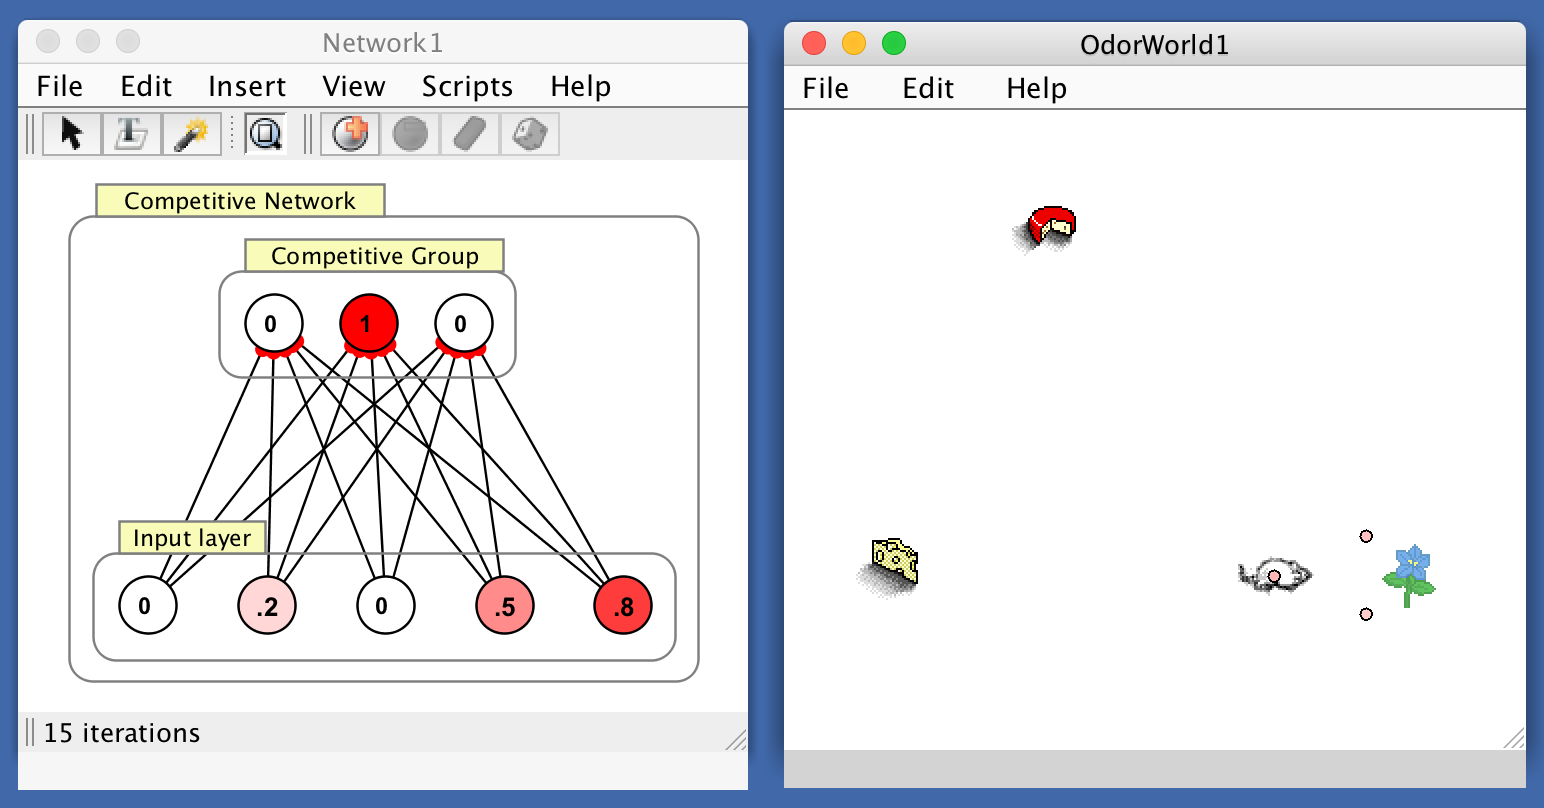
\includegraphics[scale=.4]{./images/competitive_3.png}
\caption[Simbrain screenshot]{Competitive network with 3 output nodes, which can learn to detect up to 3 clusters in an 5-dimensional input space. Inputs correspond to smells of flowers. Once the network has been trained, the output nodes can be labelled. Which output node ends up classifying which type of smell will change from one run to another of this network.}
\label{competitive_3}
\end{figure}

The way a competitive network learns can be understood visually in terms of the input space of the network. In Fig. \ref{competitiveInputSpace}, each blue dot corresponds to an input, and each red dot corresponds to the fan-in weights to an output node. When an input (blue dot) is fed to the network, the nearest output node (red dot) is the node that will turn on. As the network learns, the red dots move to the centers of the clusters. In this way, the output nodes become cluster detectors. 
% Link to linear algebra chapter, once normalization is added as a topic there. 

\begin{figure}[h]
\centering
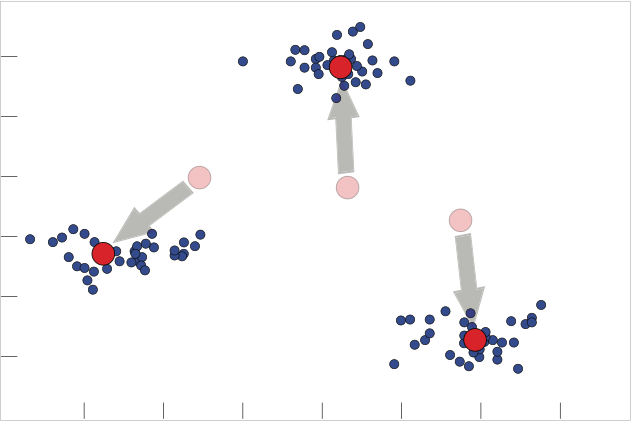
\includegraphics[scale=1]{./images/competitiveInputSpace.png}
\caption[Pamela Payne.]{Geometrical illustration of how competitive networks learn. If we think of this as a representation of the smell inputs in Fig. \ref{competitive_3}, then each blue dot corresponds to one smell from one location in the virtual world, and the three clusters correspond to the three objects: Swiss cheese, Gouda, and the blue flower. }
\label{competitiveInputSpace}
\end{figure}

Now we can say in more detail how competitive learning works. The competitive network is initialized with random weights. Thus, the red dots in Fig. \ref{competitive_3} begin at random locations in the input space. When we start to apply the algorithm, input vectors (the blue points in the input space) are presented to the network in succession. At a given iteration, whichever fan-in weight vector is closest to that input vector ``wins  the competition'' (hence the name ``competitive learning''), and that weight vector is changed in such a way that it is moved closer to that input vector in the input space. Hence, that output node will be more likely to respond to that input in the future.

% Redo  in pseudo-code / algorithm notation. 
% Week11 powerpoint has a simplified version of this
% Give the full algorithm in a footnote
% First item mention odor world case with no table?
% Add some clarification that the actual implementation of the algorithm assumes weights and inputs are both normalized, so that learning can be visualized as movement of points on a hypersphere. The original PDP discussion and Rummelhart/Zipser papers show it this way, but it easier to present things on a plane (which can be thought of as a zoomed-in region of a sphere). 
Here is the algorithm in more detail. For each row vector in the input dataset:
\begin{enumerate}
\item Use the row vector to set the input node activations.
\item Determine the winning output node, which is the output whose fan-in weight vector is closest to the input vector in the input space.\footnote{That is, the output node with the greatest weighted input.} 
\item Assign the winner a value of 1 and the losers a value of 0.
\item Move the fan-in weight vector of the winning unit towards the current input in the input space. That is, update the weights attaching to the winning neuron, so that that neuron is more likely to fire in response to the same inputs in the future.
\end{enumerate}
By repeated application of this algorithm, the fan-in weight vectors (the red dots) will incrementally move towards the input vectors closest to them. Over time, they will migrate towards the ``centers'' of the clusters in the  input space. In this case, each red dot migrates towards the center of one of the three clusters of blue dots. After training, each of the three output neurons has come to represent one cluster of inputs. Each output neuron will now fire in response to any input in the cluster around it. This shows visually the sense in which the outputs have come to represent the statistics of the input space. Each output is tuned to respond to a given cluster of inputs. 
% Idea that as one output node is tuned, it pulls _away_ from others, which then become eligible for update.

The network will also generalize well: any new input near one of the clusters will activate the neuron for that cluster. 

This process can be simulated in Simbrain using the workspace \emph{competitiveNetSmells.zip}. When you open the workspace, you will see a competitive network with four outputs and a world with 6 objects. Each object is represented by a distributed pattern of activity on the input nodes. The 6 objects---3 cheeses and 3 flowers---correspond to 6 well-separated points in the input space. With training, 6 of the 9 output nodes should begin to respond to these inputs.

Now press play and just move the mouse from object to object. The mouse is simply smelling different things in its environment and not being told how to respond (so this is a nice case of unsupervised learning). As you move the mouse around, the network will start responding to the different inputs in different ways. Eventually, it should respond to each of the different inputs with a distinct output. The output nodes get ``assigned'' to these different inputs with learning. To make this clear, you can label the nodes appropriately and verify that the network has indeed learned to separately represent the different objects. So the mouse has learned something about the statistics of its environment without any training signal, assigning a distinct representation to each of four different distributed inputs.

\subsection{Self Organizing Maps}

A more sophisticated form of competitive learning is a \glossary{Self organizing map} (or SOM). The overall idea with this architecture is the same as with a simple competitive network: inputs are compared with fan-in weight vectors, a winner is chosen, and that winning neuron's fan-in weight vector is modified so that it ``moves'' closer to the input and thus comes to represent that input. Over time the output nodes come to represent specific regions of the input space \cite{kohonen1990self}.

The new idea with a SOM is to update the weights not just around the winning node, but also in a neighborhood around the winning node. A honeycomb pattern---a hexagonal array---is used on the output layer so that all nodes are equally distant from their nearest neighbors. A special algorithm is used whereby the size of this neighborhood starts is reduced over time. The result is that \emph{nearby nodes come to represent similar inputs}. Thus, a bank of output nodes in a SOM network correspond to a kind of ``map'' of the input space. Output nodes that are near each other detect similar patterns in the input space \cite{kohonen1990self}. 

% "It has experimentally turned out to be advantageous to let Ne be very wide in the beginning and shrink monotonically with time (Fig. 2). The explanation for this may be that a wide initial Nu corresponding to a coarse spatial resolution in the learning process, first induces a rough global order in them; values, after which narrowing the Ne improves the spatial resolution of the map; the acquired global order, however, is not destroyed later on" \cite{kohonen1990self}.

% Kohonen's 1990 paper has these images of the representation as it develops. The fan-in weights slowly come to span  the input space. So at an intermediate stage of learning we _kind of_ know what's going on. Only later do we really figure it out \cite{kohonen1990self}.

\begin{figure}[h]
\centering
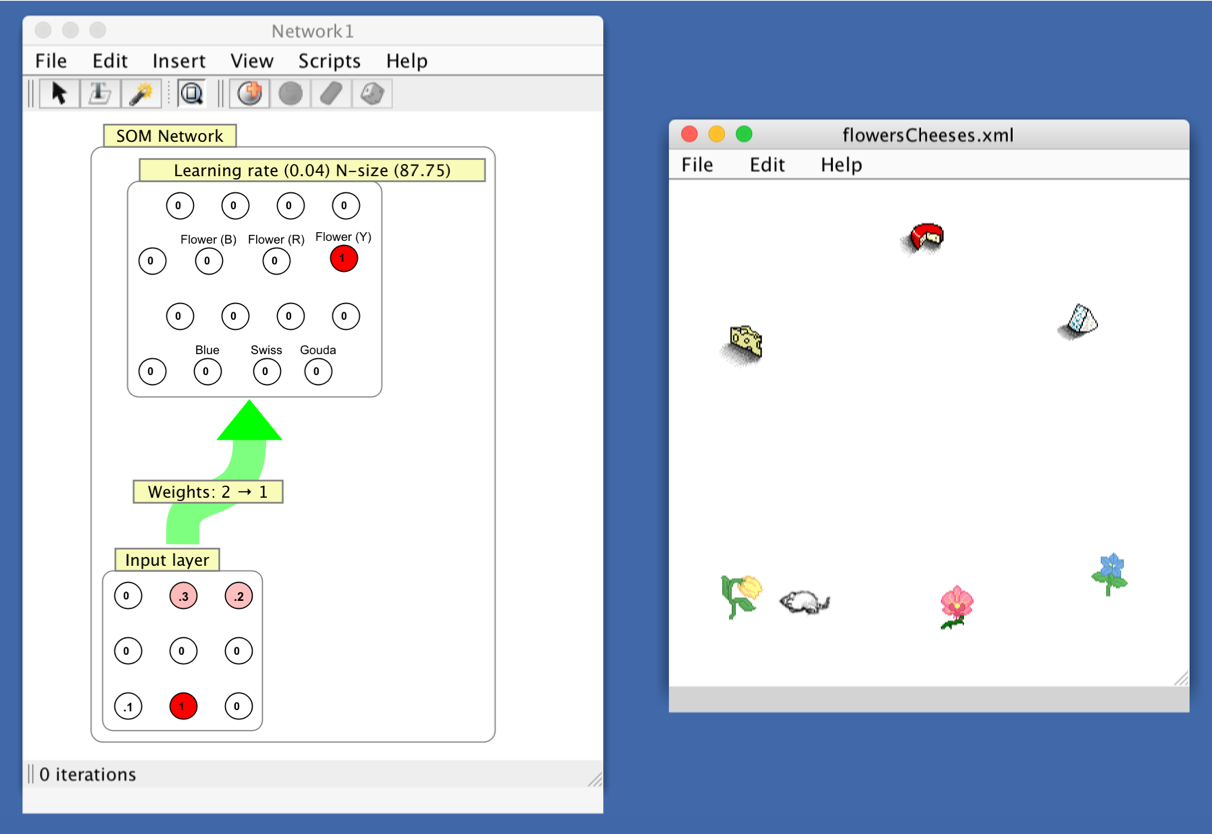
\includegraphics[scale=.5]{./images/som_labelled.png}
\caption[Simbrain screenshot.]{A self organizing map after it has been trained for several hundred iterations, with some of the categorizations it produces hand-labelled.}
% Replace cluster talk with region talk?
\label{som_labelled}
\end{figure}

Fig. \ref{som_labelled}  shows an example of a self-organizing map in Simbrain, which is based on the workspace \emph{somNetSmells.zip}. As with the simple competitive network, you can just run the network and drag the mouse around to the different objects. This simulates a sped-up process of human learning. As you run the simulation, notice that the neighborhood size (in pixels) and learning rate are being reduced. When the learning rate goes to 0, no more learning will occur, so be sure to expose the network to multiple inputs before that happens. If needed, you can right-click on the interaction box and select \emph{Reset SOM Network}. After a while, the network will stabilize. At that point, you can move the agent around to the objects, see which nodes respond to them,  and then label those nodes. I've done just that in Fig. \ref{som_labelled}. Notice that the three cheese and flower nodes are near each other in the hexagonal array of output nodes. Again, nearby nodes in the output layer correspond to nearby regions of the input space, which corresponds to objects that smell similar to each other.

SOMs are often represented only by their output nodes (that is, input nodes are omitted), since it is at the output nodes that the spatially organized maps take form. For example, in Fig. \ref{edgeDetectors} we see a top view of a large sheet of millions of neurons in the brain that are thought to behave like the output layer of a SOM, and in Fig. \ref{somSemantic} we see a top view of 150 nodes in the output nodes of a SOM.

Recall from chapter \extref{ch_neuro} that the brain is known to develop feature representations in a spatially organized way, via topographic maps. It is plausible to assume that some of these maps develop in an usupervised way over many years as a person interacts with their environment.\footnote{Though again we also saw that it can happen in a supervised way with deep networks.} In visual cortex, for example, neighboring neurons in retinotopic maps come to represent lines at similar angles  (see Fig. \ref{edgeDetectors}). In somatosensory cortex, neighboring neurons in somotatopic maps represent nearby regions of the body. In fact, spatially organized feature maps have been identified in most sensory areas of the brain. Kohonen (1990), p. 1465, reviewing the literature at the time, says:

\begin{quotation}
Some of the maps, especially those in the primary sensory areas, are ordered according to some feature dimensions of the sensory signals; for instance, in the visual areas, there are line orientation and color maps, and in the auditory cortex there are the so-called tonotopic maps, which represent pitches of tones in terms of the cortical distance, or other auditory maps. One of the sensory maps is the somatotopic map, which contains a representation of the body, i.e., the skin surface. Adjacent to it is a motor map that is topographically almost identically organized. Its cells mediate voluntary control actions on muscles. Similar maps exist in other parts of the brain. Some maps represent quite abstract qualities of sensory and other experiences. For instance, in the word-processing areas, neural responses seem to be organized according to categories and semantic values of words. It thus seems as if the internal representations of information in the brain are generally organized spatially (p. 1465; numerous citations included in the original quote are omitted here) \cite{kohonen1990self}.
\end{quotation}

\begin{figure}[h]
\centering
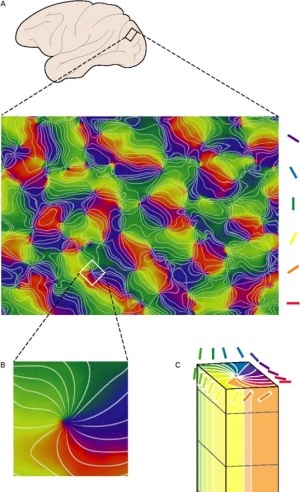
\includegraphics[scale=.6]{./images/edgeDetectorsCortex.jpg}
\caption[From \url{https://grey.colorado.edu/CompCogNeuro/index.php/File:fig_v1_orientation_cols_data.jpg}.]{Topographically organized edge detectors in visual cortex. The main panel shows a top-down view on an area of cortex, with neurons colored according to what kind of edge they represent. To the right of the panel these edge orientations are shown. Notice that nearby neurons represent similar edges, that is, edges at similar angles. From  \url{https://grey.colorado.edu/CompCogNeuro/index.php/CCNBook/Perception}.}
\label{edgeDetectors}
\end{figure}

% Add actual citation. Say something about (undoubtedly sparse) neural evidence
In more abstract regions of the brain, nearby neurons may come to represent similar \emph{concepts}. Fig. \ref{somSemantic} shows a SOM trained to model relationships between words. A network with 150 output nodes was trained on semantic data. It was trained using ``2000 presentations of word-context-pairs derived from 10,000 random sentences... Nouns, verbs, and adverbs are segregated into different domains'' (p. 1476)\cite{kohonen1990self}. Notice that nodes representing nouns, adjectives, and verbs occur in specific regions of the network, so that the network represents grammatical categories. Also note that nearby nodes represent words with similar meanings, like ``dog'' and ``horse'' or ``fast'' and ``slowly''.\footnote{Sergio Ponce de Leon refers me to this visually stunning video: \url{https://www.youtube.com/watch?v=k61nJkx5aDQ}. The point made is slightly different, and I can't speak to the merits of the study, but it is a striking way to see the general idea in action.}

\begin{figure}[h]
\centering
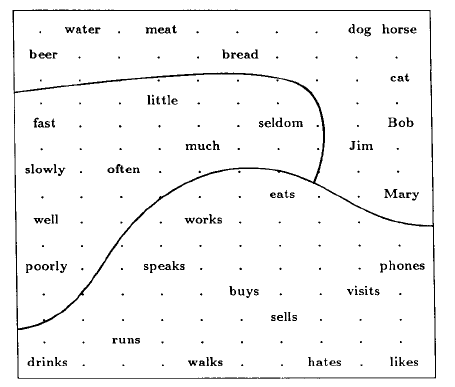
\includegraphics[scale=.5]{./images/SOM_SemanticMap.png}
\caption[From Kohonen, 1998 \cite{kohonen1990self}.]{A self organizing map trained to represent semantic features of sentences. Each dot corresponds to an output node, and labels show what concepts these nodes have learned to represent. Notice that nouns, adjectives, and verbs are represented in specific parts of the network. From Kohonen (1990), p. 1476.}
\label{somSemantic}
\end{figure}
